\documentclass{article}

\def \lastexercisenumber {21}

% ---------------------------------------------------------------- %
% short package descriptions are copied from
% https://ctan.org/

% ---------------------------------------------------------------- %

% Accept different input encodings
\usepackage[utf8]{inputenc}

% Standard package for selecting font encodings
\usepackage[T1]{fontenc}

% ---------------------------------------------------------------- %

% Multilingual support for Plain TEX or LATEX
\usepackage[english]{babel}

% ---------------------------------------------------------------- %

% Set all page margins to 1.5cm
\usepackage{fullpage}

% Margin adjustment and detection of odd/even pages
\usepackage{changepage}

% Flexible and complete interface to document dimensions
\usepackage{geometry}

% ---------------------------------------------------------------- %
% mathematics

\usepackage{amsmath}  % AMS mathematical facilities for LATEX
\usepackage{amssymb}
\usepackage{amsfonts} % TEX fonts from the American Mathematical Society
\usepackage{amsthm}   % Typesetting theorems (AMS style)

% Mathematical tools to use with amsmath
\usepackage{mathtools}

% Support for using RSFS fonts in maths
\usepackage{mathrsfs}

% Commands to produce dots in math that respect font size
\usepackage{mathdots}

% "Blackboard-style" cm fonts
\usepackage{bbm}

% Typeset in-line fractions in a "nice" way
\usepackage{nicefrac}

% Typeset quotient structures with LATEX
\usepackage{faktor}

% Vector arrows
\usepackage{esvect}

% St Mary Road symbols for theoretical computer science
\usepackage{stmaryrd}

% Three series of mathematical symbols
\usepackage{mathabx}

% ---------------------------------------------------------------- %
% algorithms

% Package for typesetting pseudocode
\usepackage{algpseudocode}

% Typeset source code listings using LATEX
\usepackage{listings}

% Reimplementation of and extensions to LATEX verbatim
\usepackage{verbatim}

% If necessary, please use the following 2 packages locally, but never both.
% This is because the algorithm environment gets defined in both packages, which leads to name conflicts.
% \usepackage{algorithm2e}
% \usepackage{algorithm}

% ---------------------------------------------------------------- %
% utilities

% A generic document command parser
\usepackage{xparse}

% Extended conditional commands
\usepackage{xifthen}

% e-TEX tools for LATEX
\usepackage{etoolbox}

% Define commands with suffixes
\usepackage{suffix}

% Extensive support for hypertext in LATEX
\usepackage{hyperref}

% Driver-independent color extensions for LATEX and pdfLATEX
\usepackage{xcolor}

% ---------------------------------------------------------------- %
% graphics

% -------------------------------- %

\usepackage{tikz}

% MISC
\usetikzlibrary{patterns}
\usetikzlibrary{decorations.markings}
\usetikzlibrary{positioning}
\usetikzlibrary{arrows}
\usetikzlibrary{arrows.meta}
\usetikzlibrary{overlay-beamer-styles}

% finite state machines
\usetikzlibrary{automata}

% turing machines
\usetikzlibrary{calc}
\usetikzlibrary{chains}
\usetikzlibrary{decorations.pathmorphing}

% -------------------------------- %

% Draw tree structures
\usepackage[noeepic]{qtree}

% Enhanced support for graphics
\usepackage{graphicx}

% Figures broken into subfigures
\usepackage{subfig}

% Improved interface for floating objects
\usepackage{float}

% Control float placement
\usepackage{placeins}

% Include PDF documents in LATEX
\usepackage{pdfpages}

% ---------------------------------------------------------------- %

% Control layout of itemize, enumerate, description
\usepackage[inline]{enumitem}

% Intermix single and multiple columns
\usepackage{multicol}
\setlength{\columnsep}{1cm}

% Coloured boxes, for LATEX examples and theorems, etc
\usepackage{tcolorbox}

% ---------------------------------------------------------------- %
% tables

% Tabulars with adjustable-width columns
\usepackage{tabularx}

% Tabular column heads and multilined cells
\usepackage{makecell}

% Publication quality tables in LATEX
\usepackage{booktabs}

% ---------------------------------------------------------------- %
% bibliography and quoting

% Sophisticated Bibliographies in LATEX
\usepackage[backend = biber, style = alphabetic]{biblatex}

% Context sensitive quotation facilities
\usepackage{csquotes}

% ---------------------------------------------------------------- %

% ---------------------------------------------------------------- %
% special letters

\newcommand{\N}{\mathbb N}
\newcommand{\Z}{\mathbb Z}
\newcommand{\Q}{\mathbb Q}
\newcommand{\R}{\mathbb R}
\newcommand{\C}{\mathbb C}
\newcommand{\K}{\mathbb K}
\newcommand{\T}{\mathbb T}
\newcommand{\E}{\mathbb E}
\newcommand{\V}{\mathbb V}
\renewcommand{\S}{\mathbb S}
\renewcommand{\P}{\mathbb P}
\newcommand{\1}{\mathbbm 1}
\newcommand{\G}{\mathbb G}

\newcommand{\iu}{\mathrm i}

% ---------------------------------------------------------------- %
% quantors

\newcommand{\Forall}        {\forall \,}
\newcommand{\Exists}        {\exists \,}
\newcommand{\nExists}       {\nexists \,}
\newcommand{\ExistsOnlyOne} {\exists! \,}
\newcommand{\nExistsOnlyOne}{\nexists! \,}
\newcommand{\ForAlmostAll}  {\forall^\infty \,}

% ---------------------------------------------------------------- %
% graphics boxed

\newcommand
{\includegraphicsboxed}
[2][0.75]
{
  \begin{center}
    \begin{tcolorbox}[standard jigsaw, opacityback = 0]

      \centering
      \includegraphics[width = #1 \textwidth]{#2}

    \end{tcolorbox}
  \end{center}
}

\newcommand
{\includegraphicsunboxed}
[2][0.75]
{
  \begin{center}
    \includegraphics[width = #1 \textwidth]{#2}
  \end{center}
}

\NewDocumentCommand
{\includegraphicsgraphicsboxed}
{ O{0.75} O{0.25} m m}
{
  \begin{center}
    \begin{tcolorbox}[standard jigsaw, opacityback = 0]

      \centering
      \includegraphics[width = #1 \textwidth]{#3} \\
      \vspace{#2 cm}
      \includegraphics[width = #1 \textwidth]{#4}

    \end{tcolorbox}
  \end{center}
}

\NewDocumentCommand
{\includegraphicsgraphicsunboxed}
{ O{0.75} O{0.25} m m}
{
  \begin{center}

    \centering
    \includegraphics[width = #1 \textwidth]{#3} \\
    \vspace{#2 cm}
    \includegraphics[width = #1 \textwidth]{#4}

  \end{center}
}

% ---------------------------------------------------------------- %
% braces

\newcommand{\pbraces}[1]{{\left  ( #1 \right  )}}
\newcommand{\bbraces}[1]{{\left  [ #1 \right  ]}}
\newcommand{\Bbraces}[1]{{\left \{ #1 \right \}}}
\newcommand{\vbraces}[1]{{\left  | #1 \right  |}}
\newcommand{\Vbraces}[1]{{\left \| #1 \right \|}}

\newcommand{\abraces}[1]{{\left \langle #1 \right \rangle}}

\newcommand{\floorbraces}[1]{{\left \lfloor #1 \right \rfloor}}
\newcommand{\ceilbraces} [1]{{\left \lceil  #1 \right \rceil }}

\newcommand{\dbbraces}    [1]{{\llbracket     #1 \rrbracket}}
\newcommand{\dpbraces}    [1]{{\llparenthesis #1 \rrparenthesis}}
\newcommand{\dfloorbraces}[1]{{\llfloor       #1 \rrfloor}}
\newcommand{\dceilbraces} [1]{{\llceil        #1 \rrceil}}

\newcommand{\dabraces}[1]{{\left \langle \left \langle #1 \right \rangle \right \rangle}}

\newcommand{\abs}  [1]{\vbraces{#1}}
\newcommand{\round}[1]{\bbraces{#1}}
\newcommand{\floor}[1]{\floorbraces{#1}}
\newcommand{\ceil} [1]{\ceilbraces{#1}}

% ---------------------------------------------------------------- %

% MISC

% metric spaces
\newcommand{\norm}[2][]{\Vbraces{#2}_{#1}}
\DeclareMathOperator{\metric}{d}
\DeclareMathOperator{\dist}  {dist}
\DeclareMathOperator{\diam}  {diam}

% O-notation
\newcommand{\landau}{{\scriptstyle \mathcal{O}}}
\newcommand{\Landau}{\mathcal{O}}

% ---------------------------------------------------------------- %

% math operators

% hyperbolic trigonometric function inverses
\DeclareMathOperator{\areasinh}{areasinh}
\DeclareMathOperator{\areacosh}{areacosh}
\DeclareMathOperator{\areatanh}{areatanh}

% special functions
\DeclareMathOperator{\id} {id}
\DeclareMathOperator{\sgn}{sgn}
\DeclareMathOperator{\Inv}{Inv}
\DeclareMathOperator{\erf}{erf}
\DeclareMathOperator{\pv} {pv}

% exponential function as power
\WithSuffix \newcommand \exp* [1]{\mathrm{e}^{#1}}

% operations on sets
\DeclareMathOperator{\meas}{meas}
\DeclareMathOperator{\card}{card}
\DeclareMathOperator{\Span}{span}
\DeclareMathOperator{\conv}{conv}
\DeclareMathOperator{\cof}{cof}
\DeclareMathOperator{\mean}{mean}
\DeclareMathOperator{\avg}{avg}
\DeclareMathOperator*{\argmax}{argmax}
\DeclareMathOperator*{\argsmax}{argsmax}

% number theory stuff
\DeclareMathOperator{\kgV}{kgV}
\DeclareMathOperator{\modulo}{mod}

% polynomial stuff
\DeclareMathOperator{\ord}{ord}

% function properties
\DeclareMathOperator{\ran}{ran}
\DeclareMathOperator{\supp}{supp}
\DeclareMathOperator{\graph}{graph}
\DeclareMathOperator{\dom}{dom}
\DeclareMathOperator{\Def}{def}
\DeclareMathOperator{\rg}{rg}

% matrix stuff
\DeclareMathOperator{\GL}{GL}
\DeclareMathOperator{\SL}{SL}
\DeclareMathOperator{\U}{U}
\DeclareMathOperator{\SU}{SU}
\DeclareMathOperator{\PSU}{PSU}
% \DeclareMathOperator{\O}{O}
% \DeclareMathOperator{\PO}{PO}
% \DeclareMathOperator{\PSO}{PSO}
\DeclareMathOperator{\diag}{diag}

% algebra stuff
\DeclareMathOperator{\At}{At}
\DeclareMathOperator{\Ob}{Ob}
\DeclareMathOperator{\Hom}{Hom}
\DeclareMathOperator{\End}{End}
\DeclareMathOperator{\Aut}{Aut}
\DeclareMathOperator{\Lin}{L}

% other function classes
\DeclareMathOperator{\Lip}{Lip}
\DeclareMathOperator{\Mod}{Mod}
\DeclareMathOperator{\Dil}{Dil}

% constants
\DeclareMathOperator{\NIL}{NIL}
\DeclareMathOperator{\eps}{eps}

% ---------------------------------------------------------------- %
% doubble & tripple powers

\newcommand
{\primeprime}
{{\prime \prime}}

\newcommand
{\primeprimeprime}
{{\prime \prime \prime}}

\newcommand
{\astast}
{{\ast \ast}}

\newcommand
{\astastast}
{{\ast \ast \ast}}

% ---------------------------------------------------------------- %
% derivatives

\NewDocumentCommand
{\derivative}
{ O{} O{} m m}
{
  \frac
  {\mathrm d^{#2} {#1}}
  {\mathrm d {#3}^{#2}}
}

\NewDocumentCommand
{\pderivative}
{ O{} O{} m m}
{
  \frac
  {\partial^{#2} {#1}}
  {\partial {#3}^{#2}}
}

\DeclareMathOperator{\Div}{div}
\DeclareMathOperator{\curl}{curl}

% ---------------------------------------------------------------- %
% integrals

\NewDocumentCommand
{\Int}
{ O{} O{} m m}
{\int_{#1}^{#2} #3 ~\mathrm d #4}

\NewDocumentCommand
{\Iint}
{ O{} O{} m m m}
{\iint_{#1}^{#2} #3 ~\mathrm d #4 ~\mathrm d #5}

\NewDocumentCommand
{\Iiint}
{ O{} O{} m m m m}
{\iiint_{#1}^{#2} #3 ~\mathrm d #4 ~\mathrm d #5 ~\mathrm d #6}

\NewDocumentCommand
{\Iiiint}
{ O{} O{} m m m m m}
{\iiiint_{#1}^{#2} #3 ~\mathrm d #4 ~\mathrm d #5 ~\mathrm d #6 ~\mathrm d #7}

\NewDocumentCommand
{\Iint}
{ O{} O{} m m m}
{\idotsint_{#1}^{#2} #3 ~\mathrm d #4 \dots ~\mathrm d #5}

\NewDocumentCommand
{\Oint}
{ O{} O{} m m}
{\oint_{#1}^{#2} #3 ~\mathrm d #4}

% ---------------------------------------------------------------- %

% ---------------------------------------------------------------- %
% amsthm-environments:

\theoremstyle{definition}

% numbered theorems
\newtheorem{theorem}             {Theorem}[section]
\newtheorem{lemma}      [theorem]{Lemma}
\newtheorem{corollary}  [theorem]{Corollary}
\newtheorem{proposition}[theorem]{Proposition}
\newtheorem{remark}     [theorem]{Remark}
\newtheorem{definition} [theorem]{Definition}
\newtheorem{example}    [theorem]{Example}
\newtheorem{heuristics} [theorem]{Heuristics}

% unnumbered theorems
\newtheorem*{theorem*}    {Theorem}
\newtheorem*{lemma*}      {Lemma}
\newtheorem*{corollary*}  {Corollary}
\newtheorem*{proposition*}{Proposition}
\newtheorem*{remark*}     {Remark}
\newtheorem*{definition*} {Definition}
\newtheorem*{example*}    {Example}
\newtheorem*{heuristics*} {Heuristics}

% ---------------------------------------------------------------- %
% exercise- and solution-environments:

% Please define this stuff in project ("main.tex"):
% \def \lastexercisenumber {...}

\newtheorem{exercise}{Exercise}
\setcounter{exercise}{\lastexercisenumber}

\newenvironment{solution}
{
  \begin{proof}[Solution]
}{
  \end{proof}
}

% ---------------------------------------------------------------- %
% MISC translations for environment-names

\renewcommand{\proofname} {Proof}
\renewcommand{\figurename}{Figure}
\renewcommand{\tablename} {Table}

% ---------------------------------------------------------------- %

\input{../../../../Fundament-LaTeX/listings.tex}

\usepackage{algorithm2e}

\addbibresource{../../../Fundament-LaTeX/references.bib}

\graphicspath{{../../../Fundament-LaTeX/images/}}

\parskip 0pt
\parindent 0pt

\title
{
  Reinforcement Learning \\
  \vspace{4pt}
  \normalsize
  \textit{Dynamic Programming}
}
\author
{
  Christian Sallinger
}
\date{3.5.2021}

\begin{document}

\maketitle

% --------------------------------------------------------------------------------

\begin{exercise}[Random walk of a robot]

A robot is placed at the origin (the point $(0, 0)$) on a two-dimension integer grid (see the figure below).
Denote the position of the robot by $(x, y)$.
The robot can either move right to $(x + 1, y)$ or move up to $(x, y + 1)$.

\begin{center}
    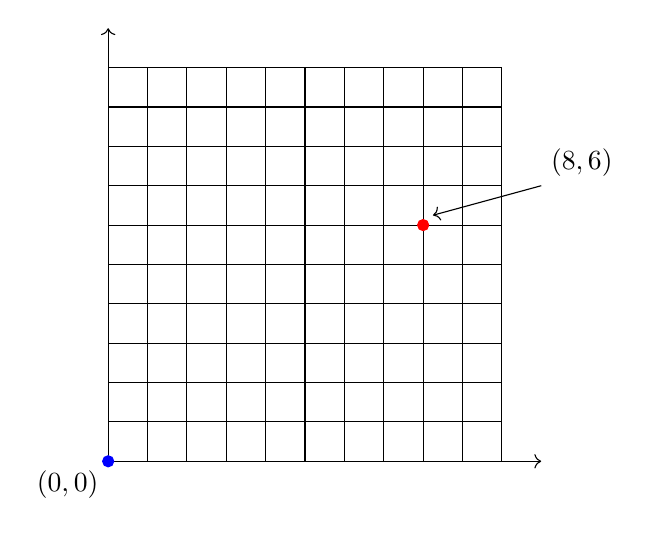
\begin{tikzpicture}[scale = 0.5]

        \draw [->] (0, 0) -- (0, 11);
        \draw [->] (0, 0) -- (11, 0);
        \draw (0, 0) grid (10, 10);

        \filldraw [color = blue] (0, 0) circle (4pt);
        \draw node [below left] {$(0, 0)$};

        \filldraw [color = red] (8, 6) circle (4pt);
        \draw [->] (11, 7) node [above right] {$(8, 6)$} -- (8.25, 6.25);

    \end{tikzpicture}
\end{center}

\begin{enumerate}[label = (\alph*)]

    \item Suppose each time the robot randomly moves right of up with equal chance.
    What is the probability that the robot will ever reach the point $(8, 6)$?

    \item Suppose another robot has a $\frac{2}{3}$ chance to move right and a $\frac{1}{3}$ chance to move up when $x + y$ is even, otherwise it has a $\frac{1}{4}$ chance to move right and a $\frac{3}{4}$ chance to move up.
    It stops whenever $|x - y| \geq 2$.
    Find the probability that $x - y = 2$ when it stops.

\end{enumerate}

\end{exercise}

% --------------------------------------------------------------------------------

\begin{solution}

\phantom{}

\begin{center}
    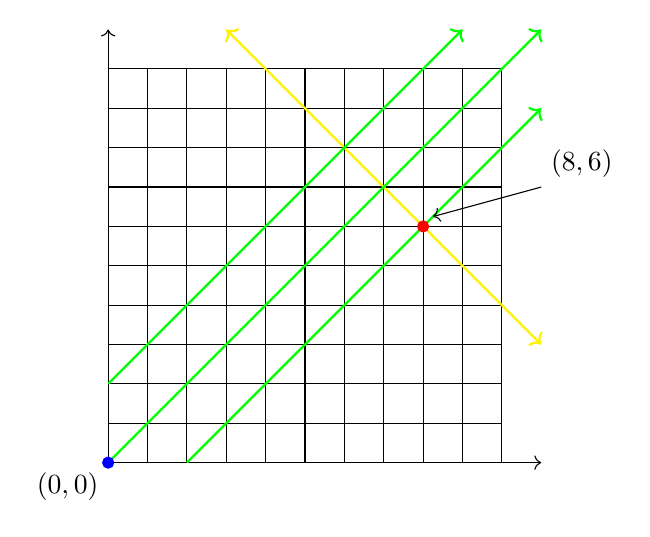
\begin{tikzpicture}[scale = 0.5]

        \draw [->] (0, 0) -- (0, 11);
        \draw [->] (0, 0) -- (11, 0);
        \draw (0, 0) grid (10, 10);

        \draw [<->, color = yellow, thick] (11, 3) -- (3, 11);

        \draw [->, color = green, thick] (0, 0) -- (11, 11);
        \draw [->, color = green, thick] (0, 2) -- (9, 11);
        \draw [->, color = green, thick] (2, 0) -- (11, 9);

        \filldraw [color = blue] (0, 0) circle (4pt);
        \draw node [below left] {$(0, 0)$};

        \filldraw [color = red] (8, 6) circle (4pt);
        \draw [->] (11, 7) node [above right] {$(8, 6)$} -- (8.25, 6.25);

    \end{tikzpicture}
\end{center}

\begin{enumerate}[label = (\alph*)]

    \item Each path that the robot moves along is equally likely.
    
    There are $\binom{a}{b}$ paths ($a = x + y$, $b \in \Bbraces{x, y}$) that lead from $(0, 0)$ to $(x, y)$.
    This can be observed by turning one of the figures above by $90 + 45$ degrees clockwise and modifying it to be a Pascal's triangle.
    The number of downwards paths that lead from the root of a Pascal's to one of its nodes with value $z$ is $z$.
    
    \begin{figure}[H]
        \centering
        \subfloat[\href{https://de.m.wikipedia.org/wiki/Datei:Pascal_triangle_small.svg}{wikipedia}]{
            \includegraphics[width = 0.35 \textwidth]{pascals_triangle_wikipedia.png}
        }
        \hspace{1cm}
        \subfloat[\href{https://stackoverflow.com/questions/47614514/how-can-i-modify-my-program-to-print-out-pascals-triangle}{stackoverflow}]{
            \includegraphics[width = 0.35 \textwidth]{pascals_triangle_stackoverflow.png}
        }
        \caption{Pascale's triangles}
    \end{figure}
    
    Let the robot move $8 + 6$ steps.
    It must land on the yellow diagonal $\Bbraces{(10, 4), \dots, (4, 10)}$.
    The position on that diagonal completely determines, whether the robot reaches $(8, 6)$ or not (since it can only move right and up).
    Consider the Binomial Theorem for $(1 + 1)^n$.
    
    \begin{align*}
        P(\text{robot passes through $(8, 6)$})
        & =
        P(\text{robot sits on $(8, 6)$} \mid \text{robot moved exactly $8 + 6$ steps}) \\
        & =
        \frac
        {
            \binom{14}{7 \pm 1}
        }{
            \sum_{n=0}^{14}
                \binom{14}{n}
        } \\
        & =
        \frac{\binom{14}{7 \pm 1}}{2^n} \\
        & \approx
        0.183288574219
    \end{align*}

    \item On the middle green diagonal $\Bbraces{(x, x)}_{x=0}^{10}$ every element $(x, x)$ has an even value $x + x$.

    $\Forall x = 0, \dots, 8:$

    \begin{align*}
        &
        P(\text{robot will move to $(x+1, x+1)$} \mid \text{robot sits at $(x, x)$}) \\
        & =
        P(\text{robot will move up and then right} \mid \text{robot sits at $(x, x)$}) \\
        & +
        P(\text{robot will move right and then up} \mid \text{robot sits at $(x, x)$}) \\
        & =
        \frac{1}{3} \frac{1}{4} + \frac{2}{3} \frac{3}{4} \\
        & =
        \frac{7}{12} =: p_0,
    \end{align*}

    \begin{align*}
        P(\text{robot will move to $(x+2, x)$} \mid \text{robot sits at $(x, x)$})
        =
        \frac{1}{3} \frac{3}{4}
        =
        \frac{3}{12} =: p_{-1},
    \end{align*}

    \begin{align*}
        P(\text{robot will move to $(x, x+2)$} \mid \text{robot sits at $(x, x)$})
        =
        \frac{2}{3} \frac{1}{4}
        =
        \frac{2}{12} =: p_1
    \end{align*}

    \begin{multline*}
        \pi_n
        :=
        P(\text{ending position $(x, y)$ fulfills $x - y = 2$} \mid x + y \leq 2 n) \\
        \xrightarrow{n \to \infty}
        P(\text{ending position $(x, y)$ fulfills $x - y = 2$}) =: \pi_\infty
    \end{multline*}

    \begin{align*}
        \pi_1 & = p_1 \\
        \pi_2 & = \pi_1 + p_0 p_1 = p_1 + p_0 p_1 = p_1 (1 + p_1) \\
        \pi_3 & = \pi_2 + p_0^2 p_1 = p_1 (1 + p_0) + p_0^2 p_1 = p_1 (1 + p_0 + p_0^2) \\
        & \vdots \\
        \pi_\infty & = p_1 \sum_{k=0}^\infty p_0^k = \frac{p_1}{1 - p_0} = \frac{2 / 12}{1 - 7 / 12} = \frac{2 / 12}{5 / 12} = \frac{2}{5} = 0.4
    \end{align*}

    \begin{comment}

        \begin{align*}
            &
            P(\text{ending position $(x, y)$ fulfills $|x - y| \neq 2$}) \\
            & =
            P
            \pbraces
            {
                \begin{array}{l}
                    \text{ending position is $(10, 10)$ and} \\
                    \text{robot only moves between diagonals $\Bbraces{(x+2, x)}_{x=0}^8$ and $\Bbraces{(x, x+2)}_{x=0}^8$}
                \end{array}
            } \\
            & =
            \underbrace
            {
                P(\text{robot will move to $(10, 10)$} \mid \text{robot sits at $(9, 9)$})
            }_1 \\
            & \quad
            P(\text{robot will move to $(9, 9)$} \mid \text{robot sits at $(8, 8)$}) \\
            & \quad
            \vdots \\
            & \quad
            P(\text{robot will move to $(1, 1)$} \mid \text{robot sits at $(0, 0)$}) \\
            & =
            \prod_{x=0}^8
                P(\text{robot will move to $(x+1, x+1)$} \mid \text{robot sits at $(x, x)$}) \\
            & =
            \pbraces{\frac{7}{12}}^9
        \end{align*}

        \begin{align*}
            P(\text{ending position $(x, y)$ fulfills $x - y = 2$})
            =
            P(\text{ending position $(x, y)$ fulfills $|x - y| = 2$}) / 2
            =
            \pbraces{1 - \pbraces{\frac{7}{12}}^9} / 2
            \approx
            0.496089600308
        \end{align*}

    \end{comment}

\end{enumerate}

\end{solution}

% --------------------------------------------------------------------------------

% -------------------------------------------------------------------------------- %

\begin{exercise}

Zeigen Sie:

\begin{enumerate}[label = (\alph*)]

    \item Bekanntlich ist die Funktion
    
    \begin{align*}
        f(x)
        =
        \begin{cases}
            \sin(1 / x) & \text{für}~ x > 0 \\
            0         & \text{für}~ x = 0
        \end{cases}
    \end{align*}

    Im Intervall $[0, 1]$ Riemann-integrierbar.
    Zeigen Sie

    \begin{align*}
        g(x)
        =
        \Int[0][x]{f(u)}{u}
        =
        x^2 \cos(1 / x) - \Int[0][x]{2 u \cos(1/u)}{u}
    \end{align*}

    und damit $g^\prime(x) = f(x)$ für alle $x \in [0, 1]$ (wobei in $0$ eigentlich nur die einseitige Ableitung existiert, Sie können sich aber vorstellen, dass $g$ (und $f$) auf er negativen Achse einfach null sind.)

    \item Für $a > 0$ wählen wir $n$ so, dass
    
    \begin{align*}
        \frac{1}{n \pi} < \frac{a}{2}
    \end{align*}

    gilt.
    Dann ist für $a > 0$ die Funktion

    \begin{align*}
        h_{0, a}(x)
        =
        \begin{cases}
            g(x)               & \text{für}~ 0 \leq x \leq \frac{1}{n \pi}, \\
            g(\frac{1}{n \pi}) & \text{für}~ \frac{1}{n \pi} < x < a - \frac{1}{n \pi}, \\
            g(a - x)           & \text{für}~ a - \frac{1}{n \pi} \leq x \leq a, \\
            0                  & \text{sonst}
        \end{cases}
    \end{align*}

    überall differenzierbar, die Ableitung $h_{0, a}^\prime$ ist überall stetig außer in den Punkten $0$ und $a$, und in jeder Umbegung von $0$ und $a$ gibt es Punkte mit $h^\prime = 1$ und $h^\prime = -1$.

    \item $h_{a, b}(x) = h_{0, b - a}(x - a)$ ist überall differenzierbar mit einer Ableitung, die überall stetig ist, außer in den Punkten $a$ und $b$ (es soll natürlich $a < b$ gelten.)

\end{enumerate}

\end{exercise}

% -------------------------------------------------------------------------------- %

\begin{solution}

\phantom{}

\begin{enumerate}[label = (\alph*)]

    \item Die linke und rechte Seite verschwinden beide für $x \to 0$.
    Weiters stimmen ihre Ableitungen in $x \in ]0, 1]$ überein.
    Unter Verwendung des rechtsseitigen Differentialquotienten, und dieser Identität, zeigt man unmittelbar $g^\prime(0) = 0$.

    \item Zwischen den Sprüngen ist die Funktion offensichtlich stetig differenzierbar.
    Darauf verschwinden die jeweiligen linksseitigen und rechtsseitigen Differentialquotienten, stimmen also insbesondere überein.

    Sei $\epsilon > 0$ hinreichend klein.

    \begin{align*}
        \implies
        \Forall x \in B_\epsilon(0) \cap (0, a):
            h_{0, 1}^\prime(x)
            =
            g^\prime(x)
            =
            f(x)
            =
            \sin(1 / x)
            \stackrel{!}{=}
            \pm 1
    \end{align*}

    Letztere Gleichheit gilt für $x := \pm \frac{1}{m \pi}$ und $m \in \N$ hinreichend groß.
    Analoges Spiel gilt für eine $\epsilon$-Umgebung von $a$.

    \item Nachdem $h_{a, b}$ eine affine Transformation der Funktion aus (b) ist, übertragen sich alle Regularitätseigenschaften.

\end{enumerate}

\end{solution}

% -------------------------------------------------------------------------------- %

% --------------------------------------------------------------------------------

\begin{exercise}

\phantom{}

\begin{enumerate}[label = (\roman*)]
    \item Zeigen Sie, dass die Funktion
    
    \begin{align*}
        f(x)
        =
        \begin{cases}
            \ln{|x|} & x \neq 0 \\
            0        & x = 0
        \end{cases}
    \end{align*}

    eine reguläre Distribution definiert, die punktweise Ableitung

    \begin{align*}
        f^\prime(x)
        =
        \begin{cases}
            \frac{1}{x}        & x \neq 0 \\
            \text{undefiniert} & x = 0
        \end{cases}
    \end{align*}

    jedoch nicht.

    \item Es bezeichne $\pv{(\frac{1}{x})}$ die Distribution
    
    \begin{align*}
        \langle \pv{\pbraces{\frac{1}{x}}}, \varphi \rangle
        =
        \lim_{\varepsilon \to 0+}
        \pbraces
        {
            \Int[-\infty][-\varepsilon]
            {
                \frac{\varphi(x)}{x}
            }{x}
            +
            \Int[\varepsilon][\infty]
            {
                \frac{\varphi(x)}{x}
            }{x}
        }
        =
        \lim_{\varepsilon \to 0+}
        \Int[|x| > \varepsilon]
        {
            \frac{\varphi(x)}{x}
        }{x}.
    \end{align*}

    Zeigen Sie, dass $\abraces{\pv{(\frac{1}{x})}, \varphi} = \Int[0][\infty]{\frac{\varphi(x) - \varphi(-x)}{x}}{x}$.

    \item Überprüfen Sie, dass $(\ln{|x|})^\prime = \pv{(\frac{1}{x})}$ in $\mathcal{D}^\prime(\R)$ gilt.

\end{enumerate}

\end{exercise}

% --------------------------------------------------------------------------------

\begin{solution}
\phantom{}
\begin{enumerate}[label = (\roman*)]
	\item Gegeben sei eine beliebige kompakte Menge $K \subseteq \R$. Wir wählen $a \in [1, \infty]$ mit $K \subseteq [-a, a]$. Nun ist
	\begin{align*}
	\int_K \vbraces{f(x)} dx &\leq 2 \pbraces{\int_1^a \log(x) dx - \int_0^1 \log(x) dx} \\
	&= 2 \pbraces{(\log(a)a - a) - (\log(1)1 - 1) - \pbraces{(\log(1)1 - 1) - \lim_{\epsilon \to 0+} (\log(\epsilon)\epsilon - \epsilon )}} \\
	&= \log(a)a - a + 2 < \infty.
	\end{align*}
	Betrachte hingegen 
	\begin{align*}
	\int_0^1 \vbraces{f^\prime(x)} dx = \int_0^1 \frac{1}{x} dx = \log(1) - \lim_{\epsilon \to 0+} \log(\epsilon) = \infty.
	\end{align*}
	\item Wir berechnen
	\begin{align*}
	\abraces{\pv\pbraces{\frac{1}{x}}, \phi} &= \lim_{\varepsilon \to 0+}
	\pbraces
	{
		\Int[-\infty][-\varepsilon]
		{
			\frac{\varphi(t)}{t}
		}{t}
		+
		\Int[\varepsilon][\infty]
		{
			\frac{\varphi(x)}{x}
		}{x}
	} \\
	&= \lim_{\varepsilon \to 0+}
	\pbraces
	{
	-\Int[\varepsilon][\infty]
	{
		\frac{\varphi(-x)}{x}
	}{x}
	+
	\Int[\varepsilon][\infty]
	{
		\frac{\varphi(x)}{x}
	}{x}
	} = \Int[0][\infty]{\frac{\varphi(x) - \varphi(-x)}{x}}{x}
	\end{align*}
	\item 
	\begin{align*}
	\abraces{\pbraces{\log|x|}^\prime, \phi} &= -\abraces{\log|x|, \phi^\prime} = -\Int[\R][]{\log|x| \phi^\prime(x)}{x} = -\Int[0][\infty]{\log|x| (\phi^\prime(x) + \phi^\prime(-x))}{x} \\
	&= -\Int[0][\infty]{\log|x| (\phi(x) - \phi(-x))^\prime}{x} = \Int[0][\infty]{\frac{\varphi(x) - \varphi(-x)}{x}}{x} = \abraces{\pv\pbraces{\frac{1}{x}}, \phi}
	\end{align*}
\end{enumerate}

\end{solution}

% --------------------------------------------------------------------------------

% --------------------------------------------------------------------------------

\begin{exercise}

Zeigen Sie, dass

\begin{align*}
    \lim_{\varepsilon \to 0+}
    \frac{1}{x - i \varepsilon}
    =
    \pv
    {
        \pbraces
        {
            \frac{1}{x}
        }
    }
    +
    \pi i \delta.
\end{align*}

\end{exercise}

% --------------------------------------------------------------------------------

\begin{solution}

Wir beginnen mit der Rechnung 
\begin{align*}
\frac{1}{x - i\varepsilon} = \frac{x + i \varepsilon}{x^2 + \varepsilon^2} = \frac{x}{x^2 + \varepsilon^2} + i\frac{\varepsilon}{x^2 + \varepsilon^2}.
\end{align*}
Gegen was der zweite Summand konvergiert wissen wir schon aus der zweiten Aufgabe. K"ummern wir uns also um den Ersten. Könnten wir beispielsweise für ein beliebiges $\phi \in \mathcal{D}(\R)$ zeigen, dass (evtl Satz von der monotonen Konvergenz?)
\begin{align*}
\lim_{\varepsilon \to 0+} \abraces{\log\pbraces{\sqrt{x^2 + \varepsilon^2}}, \phi}&= \lim_{\varepsilon \to 0+} \Int[\R][]{\log\pbraces{\sqrt{x^2 + \varepsilon^2}} \phi(x)}{x} = \Int[\R][]{\lim_{\varepsilon \to 0+}\log\pbraces{\sqrt{x^2 + \varepsilon^2}} \phi(x)}{x} = \\
&= \Int[\R][]{\log|x| \phi(x)}{x} = \abraces{\log|x|, \phi},
\end{align*}
so würde mit Lemma 3.13 schon 
\begin{align*}
\frac{x}{x^2 + \varepsilon^2} = \pbraces{\log\pbraces{\sqrt{x^2 + \varepsilon^2}}}^\prime \to \pbraces{\log|x|} = \pv\pbraces{\frac{1}{x}}
\end{align*}
folgen.
\end{solution}

% --------------------------------------------------------------------------------

% --------------------------------------------------------------------------------

\begin{exercise}[Transformations]

Suppose $X$ and $Y$ are independent gamma distributed random variables with $X \sim \operatorname{Gamma}(\alpha_1, \beta)$ and $Y \sim \operatorname{Gamma}(\alpha_2, \beta)$.
Consider the following two random variables

\begin{align*}
    U = X + Y
    \quad
    \text{and}
    \quad
    V = \frac{X}{X + Y}.
\end{align*}

\begin{enumerate}[label = (\alph*)]
    \item Show that $U \sim \operatorname{Gamma}(\alpha_1 + \alpha_2, \beta)$.
    \item Show that $U$ and $V$ are also independent random variables.
\end{enumerate}

\end{exercise}

% --------------------------------------------------------------------------------

\begin{solution}

ToDo!

\end{solution}

% --------------------------------------------------------------------------------

% --------------------------------------------------------------------------------

\begin{exercise}

Eine Distribution heißt \textit{positiv} wenn $\abraces{u, \varphi} \geq 0$ für alle $\varphi \geq 0$ gilt.

\begin{enumerate}[label = (\roman*)]
    \item Zeigen Sie, dass jede positive Distribution Ordnung $0$ hat.
    \item Zeigen Sie, dass folgende Distribution $T \in \mathcal{D}^\prime(\R)$ nicht positiv ist:
    
    \begin{align*}
        \abraces{T, \varphi}
        =
        \Int[-\infty][-1]
        {
            \frac{\varphi(x)}{|x|}
        }{x}
        +
        \Int[1][\infty]
        {
            \frac{\varphi(x)}{|x|}
        }{x}
        +
        \Int[-1][1]
        {
            \frac{\varphi(x) - \varphi(0)}{|x|}
        }{x}.
    \end{align*}

\end{enumerate}

\end{exercise}

% --------------------------------------------------------------------------------

\begin{solution}
\phantom{}
\begin{enumerate}[label = (\roman*)]
	\item Seien $K \subseteq \Omega$ und $\phi \in \mathcal{D}(K)$ beliebig.
	\item Wir wählen die Funktion 
	\begin{align*}
	\phi(x) =
	\begin{cases}
	\exp\pbraces{\frac{1}{x^2 - 1}} &, \vbraces{x} < 1 \\
	0 &, \vbraces{x} \geq 1,
	\end{cases}
	\end{align*}
	welche, wie wir aus der Vorlesung wissen, aus $\mathcal{D}(\R)$ ist und $\phi \geq 0$ erfüllt. Außerdem nimmt die Funktion im Punkt $0$ ihr Maximum an. Deshalb ist sicher
	\begin{align*}
	\abraces{T, \varphi} = \Int[-1][1]
	{
		\frac{\varphi(x) - \varphi(0)}{|x|}
	}{x} < 0 
	\end{align*}
	und damit $T$ nicht positiv.
\end{enumerate}

\end{solution}

% --------------------------------------------------------------------------------

% --------------------------------------------------------------------------------

\begin{exercise}[Exercise 4.10]

What is the analog of the value iteration update (4.10) for action values $q_{k+1}(s,a)$?

\begin{align}
  v_{k+1}(s) \ &\dot= \ \max_a \E[R_{t+1} + \gamma v_k(S_{t+1}) | S_t = s, A_t = a] \notag \\
  &= \max_a \sum_{s',r} p(s',r,a|s,a)[r + \gamma v_k(s')] \tag{4.10}.
\end{align}

\end{exercise}

% --------------------------------------------------------------------------------

\begin{solution}

\begin{align*}
  q_{k+1}(s,a) \ &\dot= \ \max_{a} \E_\pi[R_{t+1} + \gamma \sum_{a'}q_\pi(S_{t+1},a') | S_t = s, A_t = a] \\
  &= \max_{a} \sum_{s',r} p(s',r|s,a)\left[r + \gamma \sum_{a'} \pi(a'|s')q_k(s',a')\right].
\end{align*}

\end{solution}

% --------------------------------------------------------------------------------


%\printbibliography

\end{document}
